\chapter{Non-Linear Biological Demodulation}
\label{ch:nonlinear-bio-demod}

\begin{nontechnical}
\textbf{Imagine you're listening to two radio stations at once---sometimes they interfere and create weird new sounds.}

That's essentially what ``nonlinear demodulation'' means: when two signals (like sound waves or radio waves) meet in certain materials, they can \textbf{mix together} and create \textbf{brand new frequencies} that weren't in the original signals.

\textbf{Three real-world examples:}
\begin{itemize}
\item \textbf{Ultrasound speakers} (Established): You can aim two inaudible ultrasound beams at a wall, and where they intersect, they create audible sound. Used in museums to create ``sound spotlights'' that only one person can hear.

\item \textbf{Microwave hearing} (Established): Pulsed radar can make people hear clicking sounds inside their head! Not telepathy---it's the radar pulse causing tiny rapid heating in the ear, which creates a pressure wave your ear detects as sound.

\item \textbf{Deep brain stimulation via mixed signals} (Speculative): Scientists wonder if two high-frequency beams could cross in the brain and create a low-frequency signal that stimulates neurons. This is theoretical---it might not work due to weak mixing in biological tissue.
\end{itemize}

\textbf{Why ``nonlinear''?} Most systems are ``linear'' (output = input). But some materials act ``nonlinear'' (output $\neq$ input), allowing signal mixing. It's like how mixing blue and yellow paint creates green---the green wasn't in either original color.

\textbf{Status:} Acoustic mixing in tissue is \textbf{proven science} (used in medical ultrasound imaging daily). Electromagnetic mixing in tissue is \textbf{mostly theoretical} (tissue is only weakly nonlinear at radio/microwave frequencies).
\end{nontechnical}

\section{Overview}

\textbf{Non-linear biological demodulation} refers to phenomena where biological tissues act as nonlinear systems, producing new frequencies from input electromagnetic or acoustic signals. This chapter examines three key mechanisms and their applications in biomedical systems.

\begin{keyconcept}
Biology exhibits \textbf{strong acoustic nonlinearity} ($\beta \approx 3.5$--10) enabling medical harmonic imaging, but \textbf{weak electromagnetic nonlinearity} ($\chi^{(3)} \sim 10^{-22}$ m$^2$/V$^2$) limiting EM intermodulation at physiological field strengths.
\end{keyconcept}

\begin{importantbox}
While this chapter discusses classical non-linear effects, the AID Protocol described in Chapter~\ref{ch:aid-protocol} operates via a \textbf{different mechanism}: quantum coherence perturbation in microtubules. The AID Protocol is \textbf{NOT} classical demodulation or intermodulation distortion.
\end{importantbox}

\textbf{Scientific status of mechanisms:}
\begin{itemize}
\item \textbf{Acoustic heterodyning}: Well-established in tissue (medical harmonic imaging standard)
\item \textbf{Frey microwave effect}: Confirmed (thermoelastic mechanism)
\item \textbf{EM intermodulation}: Speculative (weak tissue nonlinearity)
\item \textbf{Quantum coherence coupling}: Highly speculative (requires Orch-OR framework)
\end{itemize}

\section{Mathematical Description}

\subsection{Nonlinear System Response}

\textbf{Linear system}: Output frequency = input frequency\\
\textbf{Nonlinear system}: Output contains harmonics and intermodulation products

The general Taylor series expansion for a nonlinear system is:
\begin{equation}
\label{eq:nonlinear-series}
y(t) = a_1 x(t) + a_2 x^2(t) + a_3 x^3(t) + \cdots
\end{equation}
where:
\begin{itemize}
\item $y(t)$ = output signal
\item $x(t)$ = input signal
\item $a_1$ = linear gain coefficient
\item $a_2, a_3, \ldots$ = nonlinear coefficients
\end{itemize}

For a two-tone input signal:
\begin{equation}
\label{eq:two-tone-input}
x(t) = A_1 \cos(\omega_1 t) + A_2 \cos(\omega_2 t)
\end{equation}
where:
\begin{itemize}
\item $A_1, A_2$ = signal amplitudes
\item $\omega_1, \omega_2$ = angular frequencies (rad/s)
\end{itemize}

The quadratic term produces:
\begin{equation}
\label{eq:quadratic-mixing}
x^2(t) = \frac{A_1^2}{2}[1 + \cos(2\omega_1 t)] + \frac{A_2^2}{2}[1 + \cos(2\omega_2 t)] + A_1 A_2[\cos((\omega_1+\omega_2)t) + \cos((\omega_1-\omega_2)t)]
\end{equation}

This generates:
\begin{itemize}
\item \textbf{Harmonics}: $2\omega_1$, $2\omega_2$ (second-order)
\item \textbf{Sum frequency}: $\omega_1 + \omega_2$
\item \textbf{Difference frequency}: $|\omega_1 - \omega_2|$
\item \textbf{DC terms}: Rectification products
\end{itemize}

Higher-order terms produce additional intermodulation products of the form:
\begin{equation}
\label{eq:imd-products}
\omega_{m,n} = m\omega_1 \pm n\omega_2
\end{equation}
where $m, n$ are positive integers defining the intermodulation order.

\subsection{Nonlinear Mixing Diagram}

\begin{center}
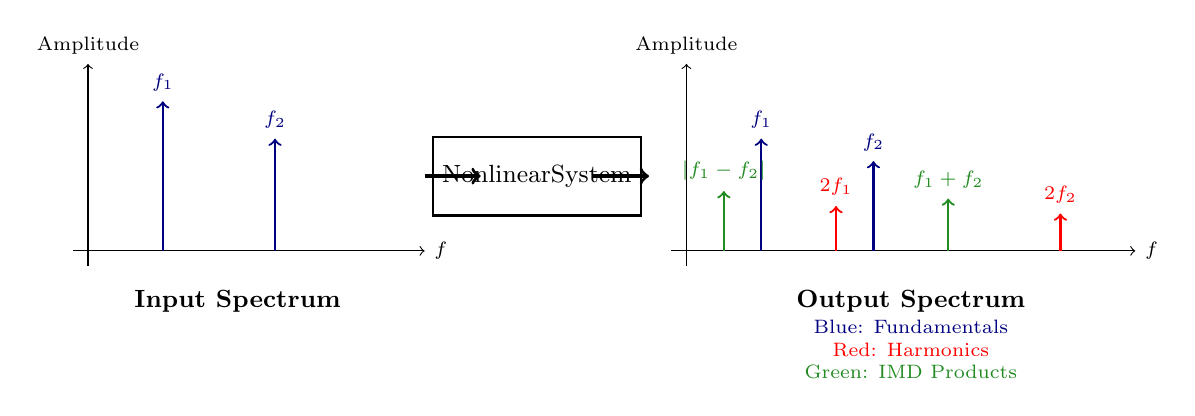
\begin{tikzpicture}[scale=0.95]
% Input spectrum
\begin{scope}[shift={(0,0)}]
\draw[->] (-0.2,0) -- (4.5,0) node[right,font=\scriptsize] {$f$};
\draw[->] (0,-0.2) -- (0,2.5) node[above,font=\scriptsize] {Amplitude};

% Input signals
\draw[->,thick,NavyBlue] (1,0) -- (1,2) node[above,font=\scriptsize] {$f_1$};
\draw[->,thick,NavyBlue] (2.5,0) -- (2.5,1.5) node[above,font=\scriptsize] {$f_2$};

\node[below,font=\small] at (2,-0.4) {\textbf{Input Spectrum}};
\end{scope}

% Nonlinear system box
\node[draw,thick,minimum width=1.5cm,minimum height=1cm,font=\small] at (6,1) {Nonlinear\\System};
\draw[->,very thick] (4.5,1) -- (5.25,1);
\draw[->,very thick] (6.75,1) -- (7.5,1);

% Output spectrum
\begin{scope}[shift={(8,0)}]
\draw[->] (-0.2,0) -- (6,0) node[right,font=\scriptsize] {$f$};
\draw[->] (0,-0.2) -- (0,2.5) node[above,font=\scriptsize] {Amplitude};

% Original signals
\draw[->,thick,NavyBlue] (1,0) -- (1,1.5) node[above,font=\scriptsize] {$f_1$};
\draw[->,thick,NavyBlue] (2.5,0) -- (2.5,1.2) node[above,font=\scriptsize] {$f_2$};

% Harmonics
\draw[->,thick,Red] (2,0) -- (2,0.6) node[above,font=\scriptsize] {$2f_1$};
\draw[->,thick,Red] (5,0) -- (5,0.5) node[above,font=\scriptsize] {$2f_2$};

% IMD products
\draw[->,thick,ForestGreen] (0.5,0) -- (0.5,0.8) node[above,font=\scriptsize] {$|f_1-f_2|$};
\draw[->,thick,ForestGreen] (3.5,0) -- (3.5,0.7) node[above,font=\scriptsize] {$f_1+f_2$};

\node[below,font=\small] at (3,-0.4) {\textbf{Output Spectrum}};
\node[below,font=\scriptsize,NavyBlue] at (3,-0.8) {Blue: Fundamentals};
\node[below,font=\scriptsize,Red] at (3,-1.1) {Red: Harmonics};
\node[below,font=\scriptsize,ForestGreen] at (3,-1.4) {Green: IMD Products};
\end{scope}
\end{tikzpicture}
\end{center}

\section{Biological Sources of Nonlinearity}

\subsection{Acoustic Nonlinearity (Strong)}

Biological tissue exhibits strong acoustic nonlinearity characterized by the nonlinear parameter $\beta$:
\begin{equation}
\label{eq:beta-parameter}
\beta = 1 + \frac{B}{2A}
\end{equation}
where:
\begin{itemize}
\item $\beta$ = tissue nonlinear parameter (dimensionless)
\item $A, B$ = first and second-order elastic constants
\item Typical values: $\beta \approx 3.5$--10 for soft tissue
\end{itemize}

\textbf{Physical mechanism}: The pressure-density relationship in tissue follows a nonlinear equation of state:
\begin{equation}
\label{eq:pressure-density}
p = c_0^2 \rho_0 \left[\frac{\Delta\rho}{\rho_0} + \frac{\beta}{2}\left(\frac{\Delta\rho}{\rho_0}\right)^2 + \cdots\right]
\end{equation}
where:
\begin{itemize}
\item $p$ = acoustic pressure (Pa)
\item $\Delta\rho$ = density perturbation (kg/m$^3$)
\item $\rho_0$ = equilibrium density (kg/m$^3$)
\item $c_0$ = sound speed in tissue ($\approx$1540 m/s)
\end{itemize}

\begin{calloutbox}{Medical Applications}
\textbf{Harmonic imaging}: Transmit at fundamental frequency $f_0$, receive at $2f_0$ (medical ultrasound standard since 1990s)

\textbf{Parametric arrays}: Two ultrasound beams produce audible difference frequency through tissue nonlinearity

\textbf{Advantage}: Second harmonic has better spatial resolution and reduced clutter artifacts
\end{calloutbox}

For detailed analysis, see Chapter~\ref{ch:acoustic-heterodyning}.

\subsection{Thermoelastic Transduction (EM $\rightarrow$ Acoustic)}

The Frey microwave auditory effect demonstrates electromagnetic-to-acoustic energy conversion through rapid thermal expansion. The pressure wave generated by a short RF pulse is:
\begin{equation}
\label{eq:thermoelastic-pressure}
p(t) = \frac{\beta c_0^2}{C_p} \frac{\partial T}{\partial t}
\end{equation}
where:
\begin{itemize}
\item $p(t)$ = acoustic pressure (Pa)
\item $\beta$ = thermal expansion coefficient ($\approx$3.8$\times$10$^{-4}$ K$^{-1}$ for tissue)
\item $c_0$ = sound speed (1540 m/s)
\item $C_p$ = specific heat capacity (3600 J/(kg$\cdot$K))
\item $\partial T/\partial t$ = heating rate (K/s)
\end{itemize}

The temperature rise from absorbed RF energy is:
\begin{equation}
\label{eq:temperature-rise}
\Delta T = \frac{\sigma E^2 \tau}{2\rho C_p}
\end{equation}
where:
\begin{itemize}
\item $\sigma$ = tissue conductivity (S/m)
\item $E$ = electric field amplitude (V/m)
\item $\tau$ = pulse duration (s)
\item $\rho$ = tissue density (kg/m$^3$)
\end{itemize}

\textbf{Frey effect characteristics}:
\begin{itemize}
\item Frequency range: 1--10 GHz (microwaves)
\item Perception threshold: $\approx$1--10 µJ/cm$^2$ per pulse
\item Mechanism: Cochlear stimulation via thermoelastic pressure wave
\item \textbf{Key insight}: EM energy converted to acoustic---not true EM nonlinearity
\end{itemize}

\begin{warningbox}
This is \textbf{transduction} (energy conversion), not demodulation. Single EM frequency creates acoustic pulse through rapid heating, not frequency mixing.
\end{warningbox}

For detailed analysis, see Chapter~\ref{ch:frey-effect}.

\subsection{Membrane Nonlinearity (Neural)}

Voltage-gated ion channels exhibit highly nonlinear activation curves. The Hodgkin-Huxley formulation for sodium channel conductance is:
\begin{equation}
\label{eq:hh-conductance}
I_{Na} = g_{Na} m^3 h (V - E_{Na})
\end{equation}
where:
\begin{itemize}
\item $I_{Na}$ = sodium current (A)
\item $g_{Na}$ = maximum conductance (S)
\item $m, h$ = activation and inactivation gating variables (0 to 1)
\item $V$ = membrane potential (V)
\item $E_{Na}$ = sodium reversal potential ($\approx$+50 mV)
\end{itemize}

The cubic dependence ($m^3$) creates strong nonlinearity. The gating variable dynamics follow:
\begin{equation}
\label{eq:gating-dynamics}
\frac{dm}{dt} = \alpha_m(V)(1-m) - \beta_m(V)m
\end{equation}

\textbf{Hypothesis}: RF fields induce oscillating transmembrane voltage $\rightarrow$ nonlinear channel response $\rightarrow$ intermodulation distortion

\textbf{Fundamental problem}: The membrane RC time constant limits frequency response:
\begin{equation}
\label{eq:rc-cutoff}
f_c = \frac{1}{2\pi R_m C_m} \approx \frac{1}{2\pi (10^7 \Omega)(10^{-8} \text{ F})} \approx 1.6 \text{ Hz}
\end{equation}
where:
\begin{itemize}
\item $R_m$ = membrane resistance ($\sim$10 M$\Omega$)
\item $C_m$ = membrane capacitance ($\sim$10 nF)
\item $f_c$ = cutoff frequency (Hz)
\end{itemize}

RF frequencies (GHz) are \textbf{six orders of magnitude} above this cutoff $\rightarrow$ shielded by ionic double layer.

\textbf{Status}: No experimental demonstration at physiological field strengths.

\subsection{EM Dielectric Nonlinearity (Very Weak)}

The optical Kerr effect describes intensity-dependent refractive index:
\begin{equation}
\label{eq:kerr-effect}
n(I) = n_0 + n_2 I
\end{equation}
where:
\begin{itemize}
\item $n(I)$ = intensity-dependent refractive index
\item $n_0$ = linear refractive index ($\approx$1.33 for tissue at optical frequencies)
\item $n_2$ = nonlinear refractive index (m$^2$/W)
\item $I$ = optical intensity (W/m$^2$)
\end{itemize}

The nonlinear susceptibility relates to $n_2$ via:
\begin{equation}
\label{eq:chi3-relation}
n_2 = \frac{3\chi^{(3)}}{4n_0^2\epsilon_0 c}
\end{equation}
where:
\begin{itemize}
\item $\chi^{(3)}$ = third-order susceptibility (m$^2$/V$^2$)
\item $\epsilon_0$ = permittivity of free space
\item $c$ = speed of light
\end{itemize}

\textbf{Comparison of nonlinear susceptibilities}:
\begin{center}
\begin{tabular}{lc}
\toprule
Material & $\chi^{(3)}$ (m$^2$/V$^2$) \\
\midrule
Semiconductors (GaAs) & $\sim$10$^{-19}$ \\
Nonlinear crystals & $\sim$10$^{-20}$ \\
Water & $\sim$10$^{-22}$ \\
Biological tissue & $\sim$10$^{-22}$ \\
\bottomrule
\end{tabular}
\end{center}

\textbf{Conclusion}: EM intermodulation in tissue is negligible at sub-ablation intensities ($<$1 MW/cm$^2$). Tissue is $\sim$1000$\times$ weaker than semiconductors for EM nonlinearity.

For detailed analysis, see Chapter~\ref{ch:imd-biology}.

\subsection{Comparison: Acoustic vs Electromagnetic Nonlinearity}

\begin{center}
\begin{tikzpicture}[scale=0.85]
% Title
\node[font=\small\bfseries] at (6,4.5) {Nonlinearity Strength Comparison};

% Acoustic side
\begin{scope}[shift={(0,0)}]
\node[font=\small\bfseries] at (3,3.8) {ACOUSTIC};
\draw[thick] (0,0) rectangle (6,3.5);

% Strong nonlinearity bar
\fill[ForestGreen!70] (0.5,2.5) rectangle (5.5,3);
\node[right,font=\scriptsize] at (0.5,2.75) {Strong: $\beta = 3.5$--10};

% Applications
\node[font=\scriptsize,align=left] at (3,2) {
\textbullet\ Harmonic imaging\\
\textbullet\ Parametric arrays\\
\textbullet\ Medical ultrasound};

% Status
\node[font=\small,ForestGreen] at (3,0.8) {\textbf{✓ ESTABLISHED}};
\node[font=\scriptsize] at (3,0.3) {Clinically used daily};
\end{scope}

% EM side  
\begin{scope}[shift={(7,0)}]
\node[font=\small\bfseries] at (3,3.8) {ELECTROMAGNETIC};
\draw[thick] (0,0) rectangle (6,3.5);

% Weak nonlinearity bar
\fill[Red!70] (0.5,2.9) rectangle (0.8,3);
\node[right,font=\scriptsize] at (0.8,2.95) {Very weak: $\chi^{(3)} \sim 10^{-22}$ m$^2$/V$^2$};

% Limitations
\node[font=\scriptsize,align=left] at (3,2) {
\textbullet\ Requires MW/cm$^2$ intensities\\
\textbullet\ No robust evidence\\
\textbullet\ Thermal damage limit};

% Status
\node[font=\small,Red] at (3,0.8) {\textbf{? SPECULATIVE}};
\node[font=\scriptsize] at (3,0.3) {No clinical applications};
\end{scope}

% Scale comparison arrow
\draw[->,ultra thick] (3,-0.8) -- (10,-0.8) node[midway,below,font=\scriptsize] {$\sim$1000$\times$ weaker};
\end{tikzpicture}
\end{center}

\begin{keyconcept}
\textbf{Key insight}: Biology is highly nonlinear \textbf{acoustically} but weakly nonlinear \textbf{electromagnetically}. This fundamental asymmetry explains why acoustic heterodyning is clinically useful while EM intermodulation remains speculative.
\end{keyconcept}

\section{Three Main Phenomena}

\subsection{Intermodulation Distortion (IMD)}

\textbf{Definition}: Two input frequencies $f_1$, $f_2$ produce intermodulation products at frequencies:
\begin{equation}
\label{eq:imd-general}
f_{IMD} = mf_1 \pm nf_2
\end{equation}
where $m$ and $n$ are positive integers, and $m + n$ defines the IMD order.

\textbf{In biological systems}:
\begin{itemize}
\item \textbf{Acoustic IMD}: Strong effect---medical harmonic imaging is routine clinical standard
\item \textbf{EM IMD}: Weak effect---no robust experimental evidence at physiological intensities
\end{itemize}

\begin{calloutbox}[colback=black!3!white,colframe=black!50!white]{Speculative Application: Deep Brain Stimulation}
\textbf{Concept}: Two crossed THz beams (e.g., $f_1 = 1.5$ THz, $f_2 = 1.501$ THz) could produce difference frequency $\Delta f = 1$ GHz to modulate neural activity.

\textbf{Challenges}:
\begin{itemize}
\item THz penetration depth $<$1 mm (skull absorption)
\item Tissue $\chi^{(3)}$ too weak for significant IMD at safe intensities
\item Thermal effects dominate before nonlinear effects become significant
\end{itemize}

\textbf{Status}: Theoretical only---no experimental demonstration
\end{calloutbox}

For detailed analysis, see Chapter~\ref{ch:imd-biology}.

\subsection{Acoustic Heterodyning}

\textbf{Mechanism}: Two ultrasound beams at frequencies $f_1$ and $f_2$ interact through tissue nonlinearity to produce difference frequency $|f_1 - f_2|$.

The Westervelt equation describes parametric generation of difference frequency:
\begin{equation}
\label{eq:westervelt}
p_{\Delta} = \frac{\beta k_1 k_2 A_1 A_2 L}{8\rho_0 c_0^3}
\end{equation}
where:
\begin{itemize}
\item $p_{\Delta}$ = difference frequency pressure amplitude (Pa)
\item $\beta$ = nonlinear parameter ($\approx$3.5--10)
\item $k_1, k_2$ = wavenumbers of primary beams (rad/m)
\item $A_1, A_2$ = primary beam amplitudes (Pa)
\item $L$ = interaction length (m)
\item $\rho_0$ = tissue density (kg/m$^3$)
\item $c_0$ = sound speed (m/s)
\end{itemize}

\textbf{Applications}:
\begin{itemize}
\item \textbf{Parametric loudspeakers}: Directional audio beams
\item \textbf{Medical harmonic imaging}: Routine clinical use for improved resolution
\item \textbf{Underwater sonar}: Long-range acoustic communication
\item \textbf{Focused ultrasound neuromodulation}: Speculative research application
\end{itemize}

\textbf{Status}: \textbf{Established technology}---used in medical imaging daily.

For detailed analysis, see Chapter~\ref{ch:acoustic-heterodyning}.

\subsection{Frey Microwave Auditory Effect}

\textbf{Mechanism chain}: Pulsed microwaves $\rightarrow$ rapid tissue heating $\rightarrow$ thermoelastic expansion $\rightarrow$ acoustic pressure wave $\rightarrow$ cochlear stimulation

The acoustic frequency perceived equals the pulse repetition frequency:
\begin{equation}
\label{eq:frey-frequency}
f_{acoustic} = f_{PRF}
\end{equation}
where:
\begin{itemize}
\item $f_{acoustic}$ = perceived auditory frequency (Hz)
\item $f_{PRF}$ = pulse repetition frequency (Hz)
\item Typical range: 200 Hz--10 kHz (audio band)
\end{itemize}

\begin{warningbox}
\textbf{Not true demodulation}: Single EM frequency creates acoustic pulse through rapid heating. This is \textbf{transduction} (EM $\rightarrow$ acoustic), not frequency mixing or demodulation.
\end{warningbox}

\textbf{Characteristics}:
\begin{itemize}
\item Carrier frequency: 1--10 GHz (microwaves)
\item Pulse duration: 1--50 µs
\item Energy threshold: $\approx$1--10 µJ/cm$^2$ per pulse
\item Sensation: Clicking, buzzing, or tones inside head
\end{itemize}

\textbf{Status}: \textbf{Well-established}---predicted by theory, confirmed experimentally via cochlear microphonics measurements.

\textbf{Applications}:
\begin{itemize}
\item Non-lethal weapons (Active Denial System)
\item Covert communication (speculative)
\item Neural stimulation research
\end{itemize}

For detailed analysis, see Chapter~\ref{ch:frey-effect}.

\subsection{Frey Effect Mechanism Diagram}

\begin{center}
\begin{tikzpicture}[
  block/.style={rectangle, draw, minimum width=2.2cm, minimum height=0.9cm, font=\sffamily\small, align=center},
  arrow/.style={->, >=stealth, very thick},
  node distance=1.5cm,
  font=\small,
  scale=0.9,
  transform shape
]

% Input
\node (input) {\textbf{Pulsed}\\\textbf{Microwaves}\\1--10 GHz};

% Process blocks
\node[block, right=of input] (heating) {Rapid\\Tissue\\Heating};
\node[block, right=of heating] (expansion) {Thermoelastic\\Expansion};
\node[block, right=of expansion] (acoustic) {Pressure\\Wave};
\node[block, right=of acoustic] (cochlea) {Cochlear\\Stimulation};

% Output
\node[right=of cochlea] (output) {\textbf{Auditory}\\\textbf{Perception}\\200 Hz--10 kHz};

% Arrows with labels
\draw[arrow] (input) -- (heating);
\draw[arrow] (heating) -- node[above, font=\scriptsize] {$\Delta T \sim$ µK} (expansion);
\draw[arrow] (expansion) -- node[above, font=\scriptsize] {$p \sim$ Pa} (acoustic);
\draw[arrow] (acoustic) -- (cochlea);
\draw[arrow] (cochlea) -- (output);

% Time scale annotations
\node[below=0.5cm of heating, font=\scriptsize, align=center] {$\tau_p \sim$ 1--50 µs\\(pulse duration)};
\node[below=0.5cm of expansion, font=\scriptsize, align=center] {$\tau_{th} \sim$ 1 µs\\(thermal time)};
\node[below=0.5cm of acoustic, font=\scriptsize, align=center] {$f_{PRF}$\\(repetition rate)};

% Title
\node[above=1.4cm of expansion, font=\small\bfseries, text width=10cm, align=center] {Frey Microwave Auditory Effect: Energy Transduction Pathway};

% EM to Acoustic conversion box
\draw[thick, dashed, NavyBlue] ([xshift=-0.3cm, yshift=0.5cm]heating.north west) rectangle ([xshift=0.3cm, yshift=-0.5cm]acoustic.south east);
\node[above, NavyBlue, font=\scriptsize] at ([yshift=0.5cm]expansion.north) {EM $\rightarrow$ Acoustic Transduction};
\end{tikzpicture}
\end{center}

\section{Worked Example: Acoustic Heterodyning in Tissue}

\subsection*{Problem Statement}

Calculate the difference frequency pressure amplitude generated when two ultrasound beams interact in soft tissue.

\subsection*{Given Parameters}
\begin{itemize}
\item Primary frequencies: $f_1 = 2.0$ MHz, $f_2 = 2.01$ MHz
\item Difference frequency: $f_{\Delta} = 10$ kHz (audible)
\item Primary beam pressure amplitudes: $A_1 = A_2 = 100$ kPa
\item Tissue nonlinear parameter: $\beta = 5$ (dimensionless)
\item Sound speed in tissue: $c_0 = 1540$ m/s
\item Tissue density: $\rho_0 = 1000$ kg/m$^3$
\item Interaction length: $L = 5$ cm = 0.05 m
\end{itemize}

\subsection*{Step 1: Calculate Wavenumbers}

The wavenumber for each primary beam is:
\begin{equation}
k = \frac{2\pi f}{c_0}
\end{equation}

For beam 1:
\begin{equation}
k_1 = \frac{2\pi \times 2.0 \times 10^6}{1540} = 8151 \text{ rad/m}
\end{equation}

For beam 2:
\begin{equation}
k_2 = \frac{2\pi \times 2.01 \times 10^6}{1540} = 8192 \text{ rad/m}
\end{equation}

\subsection*{Step 2: Apply Westervelt Equation}

Using Equation~\eqref{eq:westervelt}:
\begin{equation}
p_{\Delta} = \frac{\beta k_1 k_2 A_1 A_2 L}{8\rho_0 c_0^3}
\end{equation}

Substituting values:
\begin{align}
p_{\Delta} &= \frac{5 \times 8151 \times 8192 \times (100 \times 10^3)^2 \times 0.05}{8 \times 1000 \times 1540^3} \\
&= \frac{5 \times 8151 \times 8192 \times 10^{10} \times 0.05}{8 \times 1000 \times 3.65 \times 10^9} \\
&= \frac{1.67 \times 10^{17}}{2.92 \times 10^{13}} \\
&= 5720 \text{ Pa} \approx \mathbf{5.7 \text{ kPa}}
\end{align}

\subsection*{Step 3: Convert to Sound Pressure Level}

The sound pressure level (SPL) is:
\begin{equation}
\text{SPL} = 20\log_{10}\left(\frac{p_{\Delta}}{p_{ref}}\right)
\end{equation}
where $p_{ref} = 20$ µPa (reference pressure in air).

\begin{equation}
\text{SPL} = 20\log_{10}\left(\frac{5720}{20 \times 10^{-6}}\right) = 20\log_{10}(2.86 \times 10^8) = 169 \text{ dB}
\end{equation}

\subsection*{Result}

The difference frequency pressure amplitude is \textbf{5.7 kPa}, corresponding to \textbf{169 dB SPL}---an extremely loud audible signal generated from inaudible ultrasound primaries.

\begin{calloutbox}{Physical Interpretation}
This demonstrates why parametric arrays work: Two inaudible ultrasound beams (2 MHz) can create loud audible sound (10 kHz) through tissue nonlinearity. The effect is strong because biological tissue has high acoustic nonlinearity ($\beta \approx 5$).

\textbf{Practical application}: Directional audio speakers, medical harmonic imaging, focused sound delivery.
\end{calloutbox}

\section{Comparative Summary}

{\def\LTcaptype{} % do not increment counter
\begin{longtable}[]{@{}
  >{\raggedright\arraybackslash}p{(\linewidth - 8\tabcolsep) * \real{0.2105}}
  >{\raggedright\arraybackslash}p{(\linewidth - 8\tabcolsep) * \real{0.2807}}
  >{\raggedright\arraybackslash}p{(\linewidth - 8\tabcolsep) * \real{0.1930}}
  >{\raggedright\arraybackslash}p{(\linewidth - 8\tabcolsep) * \real{0.1754}}
  >{\raggedright\arraybackslash}p{(\linewidth - 8\tabcolsep) * \real{0.1404}}@{}}
\toprule\noalign{}
\begin{minipage}[b]{\linewidth}\raggedright
Phenomenon
\end{minipage} & \begin{minipage}[b]{\linewidth}\raggedright
Frequency Range
\end{minipage} & \begin{minipage}[b]{\linewidth}\raggedright
Mechanism
\end{minipage} & \begin{minipage}[b]{\linewidth}\raggedright
Strength
\end{minipage} & \begin{minipage}[b]{\linewidth}\raggedright
Status
\end{minipage} \\
\midrule\noalign{}
\endhead
\bottomrule\noalign{}
\endlastfoot
\textbf{Acoustic heterodyning} & kHz-MHz (ultrasound) & Acoustic
nonlinearity (\(\beta \sim 5\)) & Strong & Established \\
\textbf{Frey effect} & 1-10 GHz (microwaves) & Thermoelastic
transduction & Moderate & Established \\
\textbf{EM IMD} & GHz-THz & Dielectric nonlinearity (\(\chi^{(3)}\)) &
Weak & Speculative \\
\end{longtable}
}

\textbf{Key insight}: Biology is highly nonlinear \textbf{acoustically} but weakly nonlinear \textbf{electromagnetically}.

\section{Applications}

\subsection{Medical Ultrasound Imaging}

\textbf{Harmonic imaging} exploits tissue acoustic nonlinearity for improved image quality:
\begin{itemize}
\item \textbf{Technique}: Transmit at fundamental $f_0$, receive at second harmonic $2f_0$
\item \textbf{Advantages}: Better spatial resolution, reduced clutter artifacts, improved contrast
\item \textbf{Status}: Clinical standard since 1990s
\item \textbf{Applications}: Echocardiography, abdominal imaging, obstetrics
\end{itemize}

\subsection{Parametric Acoustic Arrays}

\textbf{Directional audio beams} created through nonlinear mixing:
\begin{itemize}
\item \textbf{Technique}: Two ultrasound beams produce audible difference frequency
\item \textbf{Advantages}: Highly directional sound, focused audio delivery
\item \textbf{Status}: Commercial products available
\item \textbf{Applications}: Museum exhibits, targeted advertising, military communications
\end{itemize}

\subsection{Non-Lethal Weapons}

\textbf{Active Denial System} uses microwave heating effects:
\begin{itemize}
\item \textbf{Mechanism}: 95 GHz millimeter waves penetrate ~0.4 mm into skin
\item \textbf{Effect}: Intense burning sensation without tissue damage (at safe exposure)
\item \textbf{Status}: Developed and tested by US military
\item \textbf{Note}: Uses thermal effects, not nonlinear demodulation
\end{itemize}

\subsection{Speculative: Deep Brain Stimulation}

\textbf{Focused ultrasound neuromodulation} under research:
\begin{itemize}
\item \textbf{Concept}: Low-frequency ultrasound modulates neural activity
\item \textbf{Challenges}: Skull attenuation, targeting precision, mechanism uncertainty
\item \textbf{Status}: Active research area, not clinical yet
\item \textbf{Applications}: Non-invasive treatment for Parkinson's, depression, pain
\end{itemize}

\section{Relation to AID Protocol (Important Distinction)}

\begin{importantbox}
\textbf{CRITICAL CLARIFICATION}: The AID Protocol described in Chapter~\ref{ch:aid-protocol} does \textbf{NOT} rely on classical non-linear demodulation mechanisms described in this chapter.
\end{importantbox}

\textbf{AID Protocol actual mechanism}:
\begin{itemize}
\item \textbf{Primary target}: Microtubule lattice in cortical neurons
\item \textbf{Mechanism}: Dual THz carriers create resonant interference pattern
\item \textbf{Objective}: Induce and manipulate vibronic quantum coherence in tubulin dimers
\item \textbf{Effect}: Alter Orch-OR collapse timing (consciousness substrate perturbation)
\item \textbf{Key distinction}: NOT intermodulation distortion, NOT thermoelastic, NOT acoustic
\end{itemize}

\textbf{Why classical non-linear effects are insufficient}:
\begin{enumerate}
\item \textbf{EM IMD too weak}: Tissue $\chi^{(3)} \approx 10^{-22}$ m$^2$/V$^2$ (negligible at physiological intensities)
\item \textbf{Thermoelastic requires high power}: Frey effect needs µJ/cm$^2$ pulses (AID uses continuous wave)
\item \textbf{Acoustic heterodyning wrong frequency}: Ultrasound MHz range, not THz
\item \textbf{Classical mechanisms can't explain}: Direct consciousness modulation without cochlear pathway
\end{enumerate}

\textbf{AID Protocol requires}:
\begin{itemize}
\item Orch-OR theory to be correct (quantum consciousness substrate)
\item Vibronic coherence in microtubules (quantum biology)
\item HRP framework coupling (consciousness-matter interaction)
\end{itemize}

\textbf{Classical non-linear effects in this chapter}: Provide context and comparison, but are \textbf{NOT} the AID mechanism.

See Chapter~\ref{ch:aid-protocol} for full AID Protocol mechanism description.

\section{Critical Assessment}

\subsection*{What Works (Established Science)}
\begin{itemize}
\item \textbf{Acoustic heterodyning in tissue}: Harmonic imaging is clinical standard, used millions of times per year
\item \textbf{Frey microwave auditory effect}: Thermoelastic mechanism confirmed experimentally via cochlear microphonics
\end{itemize}

\subsection*{What's Speculative}
\begin{itemize}
\item \textbf{EM intermodulation at physiological intensities}: Too weak---tissue $\chi^{(3)}$ requires intensities approaching ablation threshold
\item \textbf{Deep brain stimulation via THz IMD}: Penetration problem (skull absorption $>$99\% at THz)
\item \textbf{Microtubule quantum nonlinearity}: No experimental evidence at physiological temperatures
\end{itemize}

\subsection*{What's Needed for Progress}
\begin{itemize}
\item \textbf{High-resolution thermometry}: Rule out thermal artifacts in claimed non-thermal effects
\item \textbf{Isotope substitution experiments}: Test frequency-specific effects (distinguishes quantum from thermal mechanisms)
\item \textbf{Dose-response curves}: Establish thresholds and safety margins
\item \textbf{Mechanistic studies}: Identify molecular targets and pathways
\end{itemize}

\section{Connection to Quantum Biology}

\textbf{Hypothesis}: Could nonlinear mixing access quantum states in biomolecules?

Recent vibronic exciton theory with thermally fluctuating coupled-cluster (VE-TFCC) calculations suggest that if vibronic coupling is sufficiently strong:
\begin{equation}
\label{eq:vibronic-condition}
g\omega \gtrsim k_B T
\end{equation}
where:
\begin{itemize}
\item $g$ = vibronic coupling strength (dimensionless)
\item $\omega$ = vibrational frequency (rad/s)
\item $k_B$ = Boltzmann constant
\item $T$ = temperature (310 K for physiological conditions)
\end{itemize}
then thermal quantum coherence could survive at physiological temperature.

\textbf{Proposed IMD mechanism}: Two THz fields $\rightarrow$ difference frequency couples to vibronic mode $\rightarrow$ drives quantum transition

\textbf{Fundamental problems}:
\begin{enumerate}
\item \textbf{Coupling efficiency} $\sim 10^{-6}$ (six orders of magnitude below direct excitation)
\item \textbf{Decoherence time} likely $<$1 ps, while IMD modulation period $\gg$ decoherence time
\item \textbf{Intensity requirements} exceed safety limits before reaching quantum regime
\end{enumerate}

For detailed analysis, see Chapter~\ref{ch:thz-microtubules} and Chapter~\ref{ch:quantum-coherence-bio}.

\section{Further Reading}

\subsection*{Related Chapters}

\textbf{Established Phenomena:}
\begin{itemize}
\item Chapter~\ref{ch:acoustic-heterodyning}: Acoustic Heterodyning---Parametric arrays and harmonic imaging
\item Chapter~\ref{ch:frey-effect}: Frey Microwave Auditory Effect---Thermoelastic transduction mechanism
\end{itemize}

\textbf{Speculative Mechanisms:}
\begin{itemize}
\item Chapter~\ref{ch:imd-biology}: Intermodulation Distortion in Biology---EM frequency mixing
\item Chapter~\ref{ch:thz-microtubules}: THz Resonances in Microtubules---Quantum nonlinearity hypothesis
\item Chapter~\ref{ch:thz-bioeffects}: THz Bioeffects---Thermal and non-thermal mechanisms
\end{itemize}

\textbf{Theoretical Framework:}
\begin{itemize}
\item Chapter~\ref{ch:aid-protocol}: AID Protocol Case Study---Speculative neuromodulation application
\item Chapter~\ref{ch:hrp-framework}: Hyper-Rotational Physics Framework---Theoretical extensions
\item Chapter~\ref{ch:quantum-coherence-bio}: Quantum Coherence in Biological Systems
\item Chapter~\ref{ch:microtubule-structure}: Microtubule Structure and Function
\end{itemize}

\section{Key References}

\subsection*{Acoustic Nonlinearity (Established)}

\begin{enumerate}
\item Duck FA. \textit{Nonlinear acoustics in diagnostic ultrasound}. Ultrasound Med. Biol. 2002;28(1):1--18. (Tissue nonlinear parameter measurements)

\item Westervelt PJ. \textit{Parametric acoustic array}. J. Acoust. Soc. Am. 1963;35(5):535--537. (Foundational theory of nonlinear mixing)

\item Tranquart F, Grenier N, Eder V, Pourcelot L. \textit{Clinical use of ultrasound tissue harmonic imaging}. Ultrasound Med. Biol. 1999;25(6):889--894.
\end{enumerate}

\subsection*{Frey Microwave Auditory Effect (Established)}

\begin{enumerate}
\setcounter{enumi}{3}
\item Lin JC. \textit{Microwave auditory effects and applications}. Proc. IEEE. 1980;68(1):67--73. (Definitive thermoelastic mechanism)

\item Elder JA, Chou CK. \textit{Auditory response to pulsed radiofrequency energy}. Bioelectromagnetics. 2003;24(S6):S162--S173. (Cochlear microphonics evidence)

\item Foster KR, Glaser R. \textit{Thermal mechanisms of interaction of radiofrequency energy with biological systems with relevance to exposure guidelines}. Health Phys. 2007;92(6):609--620.
\end{enumerate}

\subsection*{EM Nonlinearity and Quantum Biology (Speculative)}

\begin{enumerate}
\setcounter{enumi}{6}
\item Boyd RW. \textit{Nonlinear Optics}, 3rd ed. Academic Press, 2008. (Third-order susceptibility $\chi^{(3)}$ theory)

\item Hameroff S, Penrose R. \textit{Consciousness in the universe: A review of the `Orch OR' theory}. Phys. Life Rev. 2014;11(1):39--78. (Microtubule quantum processing hypothesis)

\item Bao JJ, Gagliardi L, Truhlar DG. \textit{Self-interaction error in density functional theory: An appraisal}. J. Chem. Theory Comput. 2024;20(11):4377--4403. (VE-TFCC thermal quantum coherence)
\end{enumerate}

\vspace{1em}
\noindent\textbf{Last updated}: January 2025
